\chapter{Dimensões: componentes principais e análise fatorial}
\label{cap:dimensoes}

Quando várias variáveis descrevem aspectos relacionados, podemos perguntar se uma representação com menos dimensões ajuda a compreender o conjunto. Vamos explorar essa pergunta com análise de componentes principais, conhecida pela sigla PCA, e análise fatorial exploratória, ou AFE. Embora ambas produzam tabelas de cargas, elas respondem a perguntas diferentes.

Usaremos \texttt{exemplo\_dimensoes.csv}, com 180 registros e oito indicadores contínuos \textbf{inteiramente fictícios}. Quatro receberam o nome de planejamento e quatro de monitoramento. Esses nomes ajudam a acompanhar o exemplo; não correspondem a um instrumento validado nem a diagnósticos sobre pessoas. O capítulo anterior discute pontuação e confiabilidade; aqui, vamos examinar a estrutura das relações.

\section{Resumir variáveis ou representar fatores?}

Na PCA, construímos combinações das variáveis observadas. Se $Z_1,\ldots,Z_8$ são os indicadores padronizados, o primeiro componente é:
\[
C_1=w_{11}Z_1+w_{21}Z_2+\cdots+w_{81}Z_8.
\]
Os pesos são escolhidos para maximizar a variância desse componente, sob a restrição $\sum_jw_{j1}^2=1$. Os componentes seguintes aproveitam a variância restante em direções não correlacionadas com as anteriores. Essa ordenação se refere à solução inicial, sem rotação. O objetivo é resumir informação observada \parencite{RevelleComponentes}.

Na AFE, propomos que fatores comuns ajudem a representar as relações entre indicadores. Para dois fatores, um indicador centrado pode ser escrito como:
\[
X_j=\lambda_{j1}F_1+\lambda_{j2}F_2+\varepsilon_j.
\]
As cargas $\lambda$ relacionam o indicador aos fatores; $\varepsilon_j$ representa a parte específica não explicada pelos fatores comuns. Essa parte pode incluir características específicas e erro de medida. A unicidade não é sinônimo exclusivo de erro de digitação ou de falta de qualidade \parencite{RFatorial}.

\begin{figure}[H]
\centering
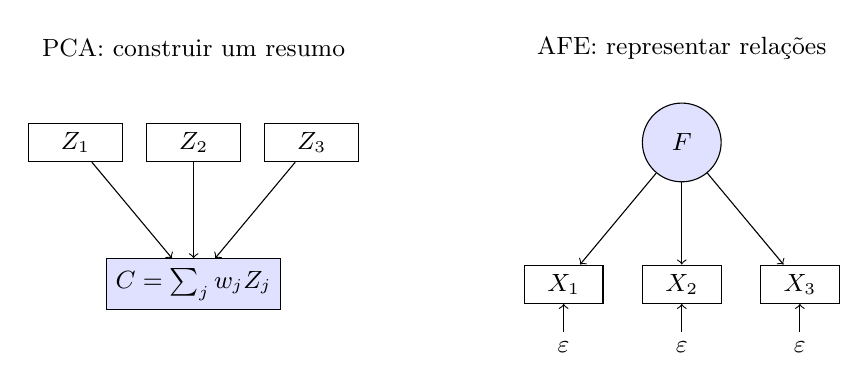
\begin{tikzpicture}[x=1cm,y=1cm,every node/.style={font=\small,align=center}]
  \node at (0,3) {PCA: construir um resumo};
  \node[draw,minimum width=1.2cm] (x1) at (-1.5,1.8) {$Z_1$};
  \node[draw,minimum width=1.2cm] (x2) at (0,1.8) {$Z_2$};
  \node[draw,minimum width=1.2cm] (x3) at (1.5,1.8) {$Z_3$};
  \node[draw,fill=blue!12,minimum width=2cm] (c) at (0,0) {$C=\sum_jw_jZ_j$};
  \draw[->] (x1)--(c); \draw[->] (x2)--(c); \draw[->] (x3)--(c);
  \node at (6.2,3) {AFE: representar relações};
  \node[draw,circle,minimum size=1cm,fill=blue!12] (f) at (6.2,1.8) {$F$};
  \node[draw,minimum width=1cm] (y1) at (4.7,0) {$X_1$};
  \node[draw,minimum width=1cm] (y2) at (6.2,0) {$X_2$};
  \node[draw,minimum width=1cm] (y3) at (7.7,0) {$X_3$};
  \draw[->] (f)--(y1); \draw[->] (f)--(y2); \draw[->] (f)--(y3);
  \foreach \a/\v in {4.7/y1,6.2/y2,7.7/y3} {
    \node (e\v) at (\a,-0.8) {$\varepsilon$}; \draw[->] (e\v)--(\v);
  }
\end{tikzpicture}
\caption{Duas perguntas de análise. As setas da PCA representam a construção matemática do resumo; as da AFE representam o modelo proposto. O desenho, sozinho, não demonstra relações causais. Elaboração própria.}
\label{fig:pca-afe-perguntas}
\end{figure}

Não devemos chamar os componentes de fatores apenas porque parecem interpretáveis. Também não basta obter dois fatores para demonstrar que existem duas características naturais bem delimitadas. Precisamos relacionar a solução à pergunta, ao conteúdo e às condições da coleta.

\section{Preparando o banco e lendo as correlações}

Abra o CSV no jamovi, defina \texttt{id} como identificador e os oito indicadores como contínuos. Não inclua o identificador na análise. Cada linha representa um registro independente. O arquivo não contém ausentes; em outros bancos, confira a regra de exclusão e o número efetivamente analisado.

Os números foram gerados com semente 20261025, duas variáveis latentes normais correlacionadas em $0{,}35$ na geração e perturbações independentes. A escala foi transformada para ficar aproximadamente em torno de 50, com dispersão próxima de 10, e arredondada a três casas. A correlação de geração não é um resultado estimado de AFE; os parâmetros foram escolhidos para construir uma atividade.

Faça primeiro uma matriz de correlações de Pearson e gráficos de dispersão. No banco, a correlação entre os dois primeiros indicadores de planejamento é aproximadamente $0{,}650$; entre o primeiro de planejamento e o primeiro de monitoramento, $0{,}304$. A figura~\ref{fig:correlacoes-dimensoes} mostra que as relações tendem a ser mais fortes dentro dos blocos, embora os blocos também se relacionem.

\begin{figure}[H]
\centering
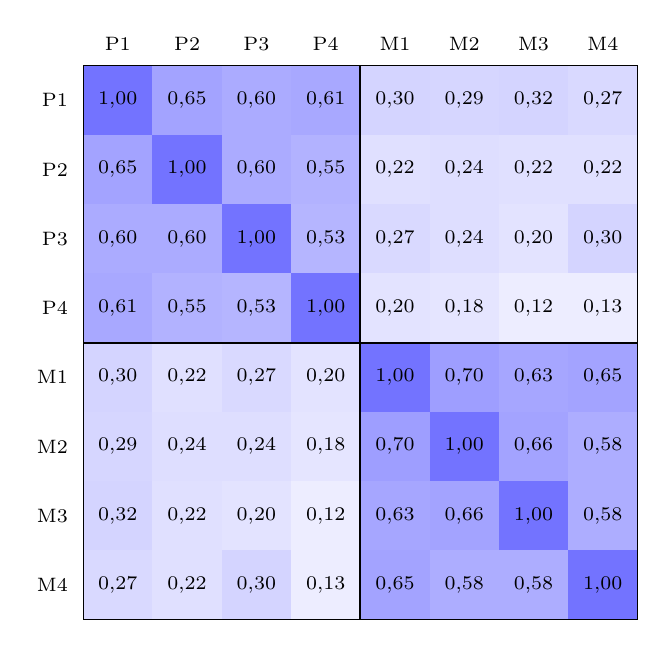
\begin{tikzpicture}[x=0.88cm,y=0.88cm,every node/.style={font=\scriptsize}]
  \fill[blue!55] (0,7) rectangle ++(1,1);
  \node at (0.5,7.5) {1,00};
  \fill[blue!36] (1,7) rectangle ++(1,1);
  \node at (1.5,7.5) {0,65};
  \fill[blue!33] (2,7) rectangle ++(1,1);
  \node at (2.5,7.5) {0,60};
  \fill[blue!34] (3,7) rectangle ++(1,1);
  \node at (3.5,7.5) {0,61};
  \fill[blue!17] (4,7) rectangle ++(1,1);
  \node at (4.5,7.5) {0,30};
  \fill[blue!16] (5,7) rectangle ++(1,1);
  \node at (5.5,7.5) {0,29};
  \fill[blue!17] (6,7) rectangle ++(1,1);
  \node at (6.5,7.5) {0,32};
  \fill[blue!15] (7,7) rectangle ++(1,1);
  \node at (7.5,7.5) {0,27};
  \fill[blue!36] (0,6) rectangle ++(1,1);
  \node at (0.5,6.5) {0,65};
  \fill[blue!55] (1,6) rectangle ++(1,1);
  \node at (1.5,6.5) {1,00};
  \fill[blue!33] (2,6) rectangle ++(1,1);
  \node at (2.5,6.5) {0,60};
  \fill[blue!30] (3,6) rectangle ++(1,1);
  \node at (3.5,6.5) {0,55};
  \fill[blue!12] (4,6) rectangle ++(1,1);
  \node at (4.5,6.5) {0,22};
  \fill[blue!13] (5,6) rectangle ++(1,1);
  \node at (5.5,6.5) {0,24};
  \fill[blue!12] (6,6) rectangle ++(1,1);
  \node at (6.5,6.5) {0,22};
  \fill[blue!12] (7,6) rectangle ++(1,1);
  \node at (7.5,6.5) {0,22};
  \fill[blue!33] (0,5) rectangle ++(1,1);
  \node at (0.5,5.5) {0,60};
  \fill[blue!33] (1,5) rectangle ++(1,1);
  \node at (1.5,5.5) {0,60};
  \fill[blue!55] (2,5) rectangle ++(1,1);
  \node at (2.5,5.5) {1,00};
  \fill[blue!29] (3,5) rectangle ++(1,1);
  \node at (3.5,5.5) {0,53};
  \fill[blue!15] (4,5) rectangle ++(1,1);
  \node at (4.5,5.5) {0,27};
  \fill[blue!13] (5,5) rectangle ++(1,1);
  \node at (5.5,5.5) {0,24};
  \fill[blue!11] (6,5) rectangle ++(1,1);
  \node at (6.5,5.5) {0,20};
  \fill[blue!17] (7,5) rectangle ++(1,1);
  \node at (7.5,5.5) {0,30};
  \fill[blue!34] (0,4) rectangle ++(1,1);
  \node at (0.5,4.5) {0,61};
  \fill[blue!30] (1,4) rectangle ++(1,1);
  \node at (1.5,4.5) {0,55};
  \fill[blue!29] (2,4) rectangle ++(1,1);
  \node at (2.5,4.5) {0,53};
  \fill[blue!55] (3,4) rectangle ++(1,1);
  \node at (3.5,4.5) {1,00};
  \fill[blue!11] (4,4) rectangle ++(1,1);
  \node at (4.5,4.5) {0,20};
  \fill[blue!10] (5,4) rectangle ++(1,1);
  \node at (5.5,4.5) {0,18};
  \fill[blue!7] (6,4) rectangle ++(1,1);
  \node at (6.5,4.5) {0,12};
  \fill[blue!7] (7,4) rectangle ++(1,1);
  \node at (7.5,4.5) {0,13};
  \fill[blue!17] (0,3) rectangle ++(1,1);
  \node at (0.5,3.5) {0,30};
  \fill[blue!12] (1,3) rectangle ++(1,1);
  \node at (1.5,3.5) {0,22};
  \fill[blue!15] (2,3) rectangle ++(1,1);
  \node at (2.5,3.5) {0,27};
  \fill[blue!11] (3,3) rectangle ++(1,1);
  \node at (3.5,3.5) {0,20};
  \fill[blue!55] (4,3) rectangle ++(1,1);
  \node at (4.5,3.5) {1,00};
  \fill[blue!38] (5,3) rectangle ++(1,1);
  \node at (5.5,3.5) {0,70};
  \fill[blue!35] (6,3) rectangle ++(1,1);
  \node at (6.5,3.5) {0,63};
  \fill[blue!36] (7,3) rectangle ++(1,1);
  \node at (7.5,3.5) {0,65};
  \fill[blue!16] (0,2) rectangle ++(1,1);
  \node at (0.5,2.5) {0,29};
  \fill[blue!13] (1,2) rectangle ++(1,1);
  \node at (1.5,2.5) {0,24};
  \fill[blue!13] (2,2) rectangle ++(1,1);
  \node at (2.5,2.5) {0,24};
  \fill[blue!10] (3,2) rectangle ++(1,1);
  \node at (3.5,2.5) {0,18};
  \fill[blue!38] (4,2) rectangle ++(1,1);
  \node at (4.5,2.5) {0,70};
  \fill[blue!55] (5,2) rectangle ++(1,1);
  \node at (5.5,2.5) {1,00};
  \fill[blue!36] (6,2) rectangle ++(1,1);
  \node at (6.5,2.5) {0,66};
  \fill[blue!32] (7,2) rectangle ++(1,1);
  \node at (7.5,2.5) {0,58};
  \fill[blue!17] (0,1) rectangle ++(1,1);
  \node at (0.5,1.5) {0,32};
  \fill[blue!12] (1,1) rectangle ++(1,1);
  \node at (1.5,1.5) {0,22};
  \fill[blue!11] (2,1) rectangle ++(1,1);
  \node at (2.5,1.5) {0,20};
  \fill[blue!7] (3,1) rectangle ++(1,1);
  \node at (3.5,1.5) {0,12};
  \fill[blue!35] (4,1) rectangle ++(1,1);
  \node at (4.5,1.5) {0,63};
  \fill[blue!36] (5,1) rectangle ++(1,1);
  \node at (5.5,1.5) {0,66};
  \fill[blue!55] (6,1) rectangle ++(1,1);
  \node at (6.5,1.5) {1,00};
  \fill[blue!32] (7,1) rectangle ++(1,1);
  \node at (7.5,1.5) {0,58};
  \fill[blue!15] (0,0) rectangle ++(1,1);
  \node at (0.5,0.5) {0,27};
  \fill[blue!12] (1,0) rectangle ++(1,1);
  \node at (1.5,0.5) {0,22};
  \fill[blue!17] (2,0) rectangle ++(1,1);
  \node at (2.5,0.5) {0,30};
  \fill[blue!7] (3,0) rectangle ++(1,1);
  \node at (3.5,0.5) {0,13};
  \fill[blue!36] (4,0) rectangle ++(1,1);
  \node at (4.5,0.5) {0,65};
  \fill[blue!32] (5,0) rectangle ++(1,1);
  \node at (5.5,0.5) {0,58};
  \fill[blue!32] (6,0) rectangle ++(1,1);
  \node at (6.5,0.5) {0,58};
  \fill[blue!55] (7,0) rectangle ++(1,1);
  \node at (7.5,0.5) {1,00};
  \foreach \x/\nome in {0.5/P1,1.5/P2,2.5/P3,3.5/P4,4.5/M1,5.5/M2,6.5/M3,7.5/M4} {
    \node[above] at (\x,8.08) {\nome};
  }
  \foreach \y/\nome in {7.5/P1,6.5/P2,5.5/P3,4.5/P4,3.5/M1,2.5/M2,1.5/M3,0.5/M4} {
    \node[left] at (-0.08,\y) {\nome};
  }
  \draw (0,0) rectangle (8,8);
  \draw[thick] (4,0)--(4,8); \draw[thick] (0,4)--(8,4);
\end{tikzpicture}
\caption{Correlações calculadas nos 180 registros fictícios. P identifica planejamento e M, monitoramento; o azul mais intenso corresponde à maior correlação positiva. Elaboração própria.}
\label{fig:correlacoes-dimensoes}
\end{figure}

Uma PCA da matriz de covariâncias considera as unidades e dispersões originais. Uma PCA da matriz de correlações equivale a trabalhar com variáveis padronizadas: cada uma entra com variância 1. Multiplicar um indicador por 100 altera sua covariância, mas não suas correlações. Para acompanhar nossos cálculos, trabalharemos com a matriz de correlações; não interprete as porcentagens abaixo como porcentagens da soma das variâncias nas unidades originais.

\section{Autovalores: quanta variância cada direção representa?}

Na matriz de correlações de oito indicadores, a variância total é 8. Os autovalores $d_1,\ldots,d_8$ indicam as variâncias dos componentes iniciais, e sua soma também é 8. A porcentagem do componente $k$ é:
\[
\%_k=100\frac{d_k}{8}.
\]
No nosso arquivo, $d_1\approx3{,}782$ e $d_2\approx1{,}912$. Assim, os dois primeiros componentes representam aproximadamente $47{,}27\%+23{,}89\%=71{,}16\%$ da variância padronizada. Os demais autovalores são aproximadamente $0{,}522$, $0{,}468$, $0{,}382$, $0{,}357$, $0{,}305$ e $0{,}273$.

Essa porcentagem descreve a representação do conjunto. Não significa que 71,16\% das pessoas foram classificadas corretamente, que a medida é 71,16\% válida ou que explicamos essa parcela de um fenômeno fora do banco.

\section{Quantas dimensões manter?}

A regra do autovalor maior que 1 compara o componente com a variância de uma variável padronizada. Neste exemplo, ela sugere dois componentes. Entretanto, oscilações amostrais também podem produzir autovalores acima de 1; a regra não deve decidir sozinha.

O \textit{scree plot} organiza os autovalores em ordem decrescente. Procuramos uma mudança de inclinação, o chamado cotovelo, para distinguir direções dominantes de uma sequência mais achatada. Esse julgamento pode ser ambíguo. A análise paralela acrescenta uma comparação com matrizes aleatórias de mesmo tamanho \parencite{RevelleParalela}.

\begin{figure}[H]
\centering
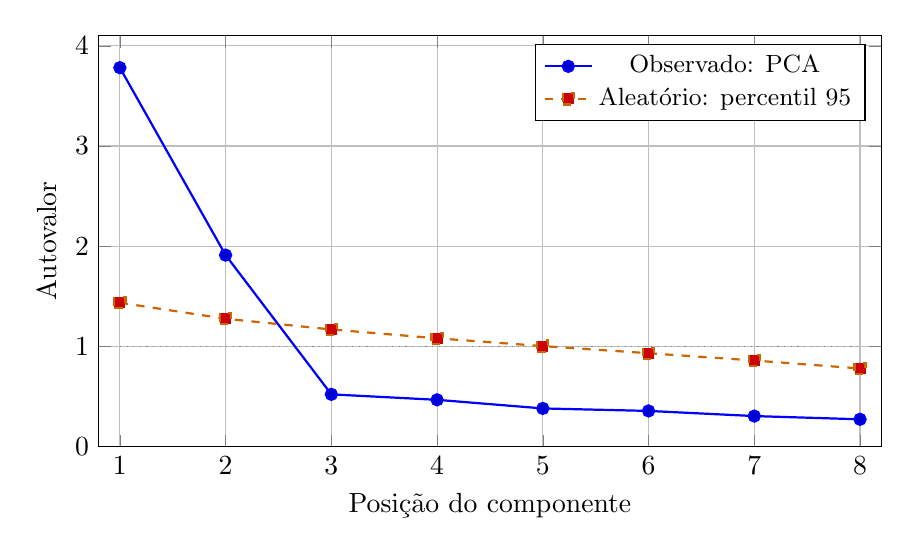
\begin{tikzpicture}
\begin{axis}[
  width=0.95\linewidth,height=6.8cm,
  xlabel={Posição do componente},ylabel={Autovalor},
  xmin=0.8,xmax=8.2,ymin=0,ymax=4.1,xtick={1,...,8},
  grid=major,legend style={font=\small,at={(0.98,0.98)},anchor=north east}]
  \addplot+[blue,thick,mark=*] coordinates {(1,3.78156122)(2,1.91150724)(3,0.52213127)(4,0.46763579)(5,0.38163977)(6,0.35685947)(7,0.30545980)(8,0.27320545)};
  \addlegendentry{Observado: PCA}
  \addplot+[orange!80!black,thick,dashed,mark=square*] coordinates {(1,1.43635315)(2,1.27669200)(3,1.16945759)(4,1.08153755)(5,1.00358333)(6,0.93256078)(7,0.85988733)(8,0.78024100)};
  \addlegendentry{Aleatório: percentil 95}
  \addplot[gray,dotted,domain=1:8] {1};
\end{axis}
\end{tikzpicture}
\caption{Autovalores do CSV e percentil 95 por posição de 2.000 matrizes normais independentes, cada uma com 180 linhas e oito colunas. Simulação própria com semente 20261026; não é reprodução da saída do jamovi. A linha pontilhada marca 1.}
\label{fig:paralela-dimensoes}
\end{figure}

Na simulação da figura, os limites dos dois primeiros componentes são aproximadamente $1{,}436$ e $1{,}277$; ambos ficam abaixo dos autovalores observados. Já o terceiro limite, $1{,}169$, fica acima de $0{,}522$. A comparação favorece dois componentes neste exercício. Simulações variam conforme a semente, o número de repetições e o critério usado.

A análise paralela para componentes e a destinada a fatores comuns não são intercambiáveis: o tratamento da diagonal e das comunalidades pode mudar o procedimento. Registre qual análise foi solicitada. Combine retenção, interpretação, resíduos e estabilidade; não aumente ou diminua fatores até conseguir apenas nomes convenientes.

\section{Executando a PCA no jamovi}

\begin{enumerate}
  \item Abra \textbf{Análises $\rightarrow$ Fator $\rightarrow$ Análise de componentes principais (Principal Component Analysis)}.
  \item Mova somente os oito indicadores para \textbf{Variables}. Solicite autovalores iniciais e \textit{scree plot}.
  \item Examine a seleção por análise paralela. Para reproduzir a tabela didática abaixo, selecione um número fixo de dois componentes e rotação \textbf{None}, isto é, sem rotação.
  \item Exiba o resumo dos componentes. Desative a ocultação de cargas pequenas, ou use limite zero, para ler a tabela inteira.
\end{enumerate}

A documentação oficial apresenta as alternativas de retenção, rotação e saídas adicionais \parencite{JamoviPCA}. Os nomes podem aparecer traduzidos conforme o idioma; os termos ingleses entre parênteses ajudam a localizar a análise.

\begin{table}[H]
\centering
\caption{Cargas calculadas da PCA de correlações, com dois componentes e sem rotação.}
\begin{tabular}{lrr}
\hline
Indicador & Componente 1 & Componente 2 \\
\hline
Planejamento 1 & $0{,}730$ & $0{,}463$ \\
Planejamento 2 & $0{,}660$ & $0{,}521$ \\
Planejamento 3 & $0{,}671$ & $0{,}468$ \\
Planejamento 4 & $0{,}583$ & $0{,}576$ \\
Monitoramento 1 & $0{,}739$ & $-0{,}468$ \\
Monitoramento 2 & $0{,}722$ & $-0{,}471$ \\
Monitoramento 3 & $0{,}694$ & $-0{,}486$ \\
Monitoramento 4 & $0{,}690$ & $-0{,}445$ \\
\hline
\end{tabular}
\label{tab:cargas-pca-dimensoes}
\end{table}

O primeiro componente acompanha os dois blocos positivamente; o segundo contrasta planejamento e monitoramento. O programa pode inverter todos os sinais de uma coluna sem mudar a solução. Além disso, carga e peso não são a mesma quantidade: nesta PCA, a carga inicial é o peso do autovetor multiplicado por $\sqrt{d_k}$. Para o primeiro indicador, $0{,}3752\sqrt{3{,}7816}\approx0{,}7296$.

\section{Da PCA à análise fatorial exploratória}

Se a pergunta é sobre uma estrutura comum aos indicadores, abra uma análise própria de \textbf{Análises $\rightarrow$ Fator $\rightarrow$ Análise fatorial exploratória (Exploratory Factor Analysis)}. Inclua os mesmos indicadores. No campo de extração, o jamovi oferece resíduos mínimos (\textbf{Minimum residual}), máxima verossimilhança e eixos principais; a escolha deve ser documentada \parencite{JamoviAFE}.

Vamos usar resíduos mínimos como ponto de partida e examinar a retenção por análise paralela para fatores. Depois, compare soluções justificáveis, como um e dois fatores, com a mesma matriz e método. Para uma solução de dois fatores, solicite rotação \textbf{Oblimin}, correlações entre fatores, resumo, medidas de ajuste e verificações KMO e Bartlett. Não use os autovalores da PCA como se fossem cargas estimadas dessa AFE.

Neste capítulo, os resultados numéricos apresentados foram calculados diretamente para a PCA. A AFE constitui uma atividade de ajuste no jamovi: registre os valores encontrados, a versão e as opções. Não fornecemos uma tabela fatorial supostamente esperada sem ajustar o modelo correspondente.

\section{Rotação: tornando a interpretação mais clara}

Uma rotação procura uma orientação mais legível da solução retida. O critério varimax foi apresentado por Kaiser como uma forma analítica de orientar as cargas; a apresentação original já discute que uma estrutura simples, isoladamente, não encerra a avaliação da solução \parencite{Kaiser1958}. \textbf{Varimax} é ortogonal: mantém fatores não correlacionados. \textbf{Oblimin} é oblíqua e permite correlação entre fatores. Permitir não significa obrigar uma correlação alta. Se as dimensões estudadas podem se relacionar, impor correlação zero precisa de justificativa \parencite{RevelleFatores}.

\begin{figure}[H]
\centering
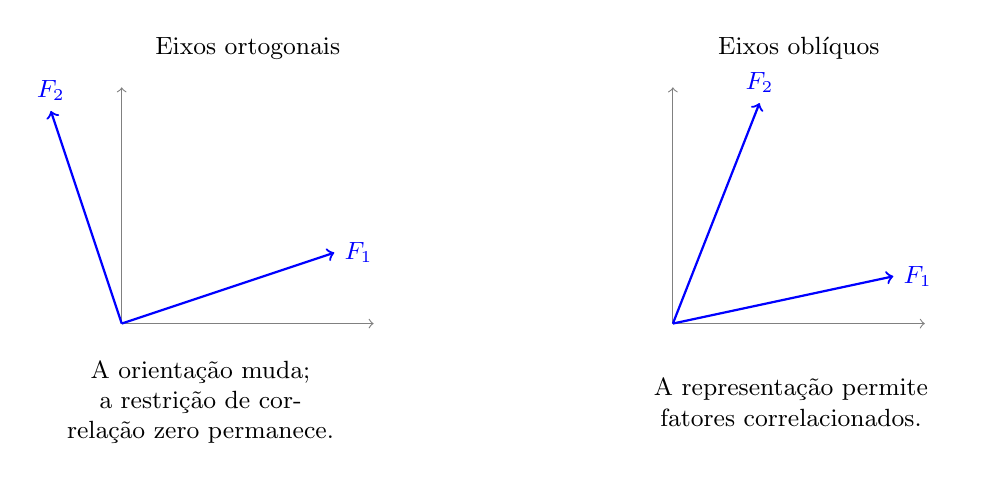
\begin{tikzpicture}[x=1cm,y=1cm,every node/.style={font=\small}]
  \begin{scope}
    \node at (1.6,3.5) {Eixos ortogonais};
    \draw[->,gray] (0,0)--(3.2,0); \draw[->,gray] (0,0)--(0,3.0);
    \draw[->,thick,blue] (0,0)--(2.7,0.9) node[right] {$F_1$};
    \draw[->,thick,blue] (0,0)--(-0.9,2.7) node[above] {$F_2$};
    \node[align=center,text width=4cm] at (1,-1) {A orientação muda;\\a restrição de correlação zero permanece.};
  \end{scope}
  \begin{scope}[xshift=7cm]
    \node at (1.6,3.5) {Eixos oblíquos};
    \draw[->,gray] (0,0)--(3.2,0); \draw[->,gray] (0,0)--(0,3.0);
    \draw[->,thick,blue] (0,0)--(2.8,0.6) node[right] {$F_1$};
    \draw[->,thick,blue] (0,0)--(1.1,2.8) node[above] {$F_2$};
    \node[align=center,text width=4cm] at (1.5,-1) {A representação permite\\fatores correlacionados.};
  \end{scope}
\end{tikzpicture}
\caption{Esquema geométrico para distinguir restrições de rotação. Os ângulos são ilustrativos e não foram calculados para o banco. Elaboração própria.}
\label{fig:rotacao-dimensoes}
\end{figure}

Em solução oblíqua, distinga a matriz padrão, com cargas que consideram os demais fatores, da matriz de estrutura, com correlações entre indicadores e fatores. Elas podem diferir. Não chame automaticamente toda carga de correlação simples, nem use a porcentagem de cada fator correlacionado como parcelas independentes que sempre se somam sem sobreposição.

\section{Cargas, comunalidades e unicidades}

Para indicadores padronizados e fatores ortogonais, a comunalidade de um indicador é a soma das cargas ao quadrado: $h_j^2=\sum_k\lambda_{jk}^2$. A unicidade é $u_j^2=1-h_j^2$. Uma carga hipotética $0{,}70$ em um único fator corresponde a $0{,}49$ de variância comum sob esse modelo. Isso não autoriza interpretar 0,70 como 70\%.

Com fatores correlacionados, a expressão geral é:
\[
h_j^2=\boldsymbol\lambda_j^{\mathsf T}\Phi\boldsymbol\lambda_j,
\]
em que $\Phi$ contém suas correlações. Para dois fatores, surge o termo cruzado $2\lambda_{j1}\lambda_{j2}\phi_{12}$; somar somente quadrados pode dar uma resposta incorreta. Por exemplo, com cargas hipotéticas $0{,}60$ e $0{,}30$ e correlação $0{,}40$, temos $h^2=0{,}36+0{,}09+0{,}144=0{,}594$.

Na nossa PCA sem rotação, a soma dos quadrados das duas cargas de planejamento 1 é aproximadamente $0{,}747$. Isso descreve a representação desse indicador pelos componentes retidos. Não transportaremos esse valor para a comunalidade de uma AFE. Cargas cruzadas, unicidades extremas ou soluções impróprias pedem investigar conteúdo, dados e modelo, em vez de apagar itens automaticamente.

\section{KMO e Bartlett: perguntas preliminares}

O KMO compara correlações simples e correlações parciais. Sua expressão global pode ser escrita como:
\[
\mathrm{KMO}=\frac{\sum_{j<k}r_{jk}^2}
{\sum_{j<k}r_{jk}^2+\sum_{j<k}r_{jk\cdot\mathrm{demais}}^2}.
\]
O valor calculado para o banco é aproximadamente $0{,}838$. Examine também os índices por indicador; um valor global pode esconder dificuldades localizadas. Não use uma classificação verbal do índice para substituir a análise do modelo \parencite{RevelleKMO}.

O teste de Bartlett examina a hipótese de uma matriz de correlações identidade. Uma aproximação é:
\[
\chi^2_B=-\left[n-1-\frac{2p+5}{6}\right]\log|R|,
\qquad gl=\frac{p(p-1)}{2}.
\]
A aproximação inferencial depende das condições do teste, incluindo independência e normalidade multivariada; o cálculo não é uma verificação dessas condições. Com $n=180$ e $p=8$, obtemos aproximadamente $686{,}04$, com 28 graus de liberdade, correspondendo a $p<0{,}001$. Rejeitar a identidade indica evidência de relações entre variáveis; não demonstra quantos fatores existem, bom ajuste ou validade \parencite{RevelleBartlett}.

\section{Escores, relato e próximos passos}

Um componente é calculado pelas combinações escolhidas. Um escore fatorial é uma estimativa de uma quantidade não observada e depende do método de estimação; ele não é o fator conhecido sem erro \parencite{RevelleEscores}. Não trate escores estimados como diagnósticos nem crie pontos de corte clínicos a partir deste exercício.

Ao relatar, informe indicadores, participantes, ausentes, matriz, retenção, extração, rotação e resultados relevantes. Um relato possível da PCA é: ``Nos 180 registros fictícios, uma PCA da matriz de correlações apresentou autovalores iniciais de 3,782 e 1,912, com 71,16\% de variância padronizada nos dois primeiros componentes. Foram examinados o gráfico de autovalores e uma simulação paralela independente. Os resultados descrevem dados construídos para ensino.''

Indicadores ordinais com poucas categorias podem exigir modelos e matrizes de correlações adequados às respostas. Mudar a medida da coluna para contínua não resolve essa questão. Antes de aplicar os procedimentos a instrumentos reais, planeje amostra, conteúdo, distribuição das respostas e avaliação em outros dados; o tamanho necessário depende da estrutura e da qualidade dos indicadores, sem uma razão universal de participantes por item.

Uma AFE desenvolvida e confirmada apenas no mesmo banco pode favorecer decisões ocasionais. Quando a estrutura orientar usos futuros, planeje avaliação em outra amostra e, se apropriado, análise confirmatória com hipóteses previamente definidas. A ligação com confiabilidade é complementar: relações fortes entre itens não demonstram, por si, a estrutura ou a interpretação pretendida.

\section{Vamos praticar: perguntas e comentários}

\begin{enumerate}
  \item Por que a soma dos oito autovalores da PCA de correlações é 8? Qual porcentagem corresponde ao primeiro?
  \item A regra do autovalor maior que 1 e a simulação paralela da figura sugerem quantos componentes? O acordo demonstra dois fatores reais?
  \item Uma carga de $0{,}70$ representa 70\% de variância comum em um modelo unifatorial padronizado?
  \item Com cargas $0{,}60$ e $0{,}30$ e correlação fatorial $0{,}40$, calcule comunalidade e unicidade.
  \item Se o jamovi inverter todos os sinais do segundo componente da tabela, a solução mudou substantivamente?
  \item O KMO de $0{,}838$ e Bartlett com $p<0{,}001$ validam um questionário? O que ainda precisamos examinar?
\end{enumerate}

\subsection*{Comentários das respostas}

\begin{enumerate}
  \item Cada variável padronizada contribui com variância 1. A soma é 8; $100(3{,}78156/8)\approx47{,}27\%$.
  \item Dois componentes no exercício. O acordo favorece uma decisão de redução, mas não demonstra a existência ou validade de fatores comuns.
  \item Não. Sob essas condições, $0{,}70^2=0{,}49$, ou 49\%.
  \item $h^2=0{,}594$ e $u^2=0{,}406$. O termo cruzado considera a correlação entre fatores.
  \item Não. Inverter o sinal de todo o componente muda sua orientação, mantendo a representação e as relações relativas.
  \item Não. Precisamos examinar conteúdo, método, retenção, cargas, resíduos, estabilidade, uso pretendido e evidências em dados apropriados. Essas verificações preliminares não substituem a avaliação completa.
\end{enumerate}


\section{Para continuar no Balaio Científico}

Como preparação para organizar os indicadores, retome os textos \href{https://www.balaiocientifico.com/2026/10/tipos-de-variaveis-no-jamovi-nominal.html}{Tipos de variáveis no Jamovi: nominal, ordinal e contínua} e \href{https://www.balaiocientifico.com/2026/10/como-criar-uma-variavel-calculada-no.html}{Como criar uma variável calculada no Jamovi: soma e média}, no blog Balaio Científico. A leitura ajuda a revisar os tipos de medida e a diferença entre colunas originais e escores calculados.

Para acompanhar visualmente o uso da calculadora, assista à aula \href{https://www.youtube.com/watch?v=NBvQphd9FqI}{Jamovi -- Calculadora Variáveis -- Aula 9}, do canal Balaio Científico. Esses materiais são pré-requisitos de preparação dos dados. O roteiro de componentes principais e análise fatorial exploratória está desenvolvido neste capítulo, com as referências oficiais indicadas ao longo do texto.
